\documentclass[journal]{IEEEtran}
\usepackage{blindtext}
\usepackage{graphicx}
\usepackage{listings}
\usepackage[superscript,biblabel]{cite}


\hyphenation{op-tical net-works semi-conduc-tor}

\begin{document}

\title{Tree Notation: an antifragile document notation}

\author{Breck~Yunits% <-this % stops a space
\thanks{Breck Yunits is a software engineer in Seattle (breck7@gmail.com).}% <-this % stops a space
}

\markboth{June~2017}%
{Shell \MakeLowercase{\textit{et al.}}: Bare Demo of IEEEtran.cls for Journals}

\maketitle


\begin{abstract}
%\boldmath
A new minimal notation is presented for encoding tree data structures. Tree Notation may be useful as a base notation for domain specific languages. A new theorem about data structures is introduced and predictions are made.

\end{abstract}

\IEEEpeerreviewmaketitle

\section{Introduction}

Many widely used applications read and write documents in a domain specific language (DSL) based on XML \cite{Bray}, JSON \cite{Crockford} or Racket. This paper and accompanying source code (github.com/breck7/treenotation) introduce a new whitespace-based notation that can serve as an alternative base notation for DSL's. These DSL's, called ETN's ("Extends Tree Notation"), are easy to create and can be very powerful. This paper describes Tree Notation (TN), three benefits, three downsides, and then introduces a new theorem arising from this notation and makes some falsifiable predictions.

\section{Tree Notation}

TN encodes one data structure, a \textbf{TreeNode}, with two members: an array of strings called \textbf{words} and an optional array of child TreeNodes called \textbf{children}.

TN defines three special characters, which in the canonical notation are node delimiter ("\textbackslash n"), node edge (" "), and word delimiter(" ").

A comparison quickly illustrates nearly the entirety of the notation:

JSON:

\begin{lstlisting}
{
 "title" : "About Ada",
 "stats": {
  "pageViews": 42
 }
}
\end{lstlisting}

Tree Notation:

\begin{lstlisting}
title About Ada
stats
 pageviews 42
\end{lstlisting}

\section{Practical Advantages}

\subsection{Easy composition}

When a document is composed of blocks written in multiple languages, those blocks may require verbose encoding to accommodate the underlying base notation.

In the example snippet below, a JSON-backed IPython notebook encodes Python to JSON. The resulting document is more complex:

\begin{lstlisting}
{
 "source": [
  "import matplotlib.pyplot as plt\n",
  "import numpy as np\n",
  "print(\"ok\")"
  ]
}
\end{lstlisting}

With TN, the Python block is indented and requires no additional transformation:

\begin{lstlisting}
source
 import matplotlib.pyplot as plt
 import numpy as np
 print("ok")
\end{lstlisting}

\subsection{Semantic diffs}

JSON, XML, and Racket serializers can encode the same object to different documents by varying whitespace. Although ignoring whitespace can be a useful feature in a language, it can also lead to large diffs--and sometimes merge conflicts--for small or non-existent semantic changes, because of different serialization implementations.

In TN, there is one and only one way to serialize an object. Diffs contain only semantic meaning. Editors and transformers can be counted on to deliver consistent results.

\subsection{Zero parse errors}

Parse errors do not exist in TN. Every document is a valid TN document. Errors can only occur at the ETN level (i.e. a mistyped property name). Typos made at the spot of a TN syntax character affect only the related node(s).

With other base notations, to get from a blank document to a certain valid document in keystroke increments requires stops at invalid documents. With TN all intermediate steps are valid.

Nodes of a document may be edited at runtime with no risk of breaking the parsing of the entire document. If a node contains an ETN error, it can fallback to an error handling node type for quick and/or automated correction.

A developer working on an editor that allows a user to edit the document source does not have to worry about handling both errors at the DSL level and errors at the base notation level. TN eliminates the latter class of errors.

\section{Drawbacks}

\subsection{Lack of Tooling and Support}

XML, JSON, and increasingly Racket are now ubiquitous, with JSON alone having over 250 widely used and well tested implementations in over 50 programming languages \cite{JSON}. TN is new, and library and application support, compared to other popular base notations, rounds to zero.

Despite the lack of widespread support at present, because of the ease of implementation and intrinsic benefits mentioned above, TN may still be worthwhile in certain applications.

\subsection{Lack of Primitive Data Types}

Some notations, such as JSON, specify notations for common primitive types like booleans and numbers. Encoded documents can then be parsed directly to the matching in-memory structures. TN is relatively minimal and delegates the encoding and decoding of additional types to ETN's. Thus parsing a TN document into the desired in-memory structures often requires the specification of an ETN.

However, in practice rarely are the primitive data structures in a base level notation like JSON enough to fully parse a structure, and usually an additional parse step is used  \cite{Ooms}.

\subsection{Cosmetic Differences}

Some developers dislike whitespace notations. In addition, without an ETN, a complex node in TN may be verbose, extending over multiple lines, with one node per line, whereas other base notations may benefit from a denser display of information out-of-the-gate, with multiple nodes per line.

\section{The Tree Theorem (TTT)}

Working with TN leads to some observations about the general nature of data. To the LISP programmer, all data structures are recursive lists (or perhaps "recursive cons"). With the introduction of TN, this general notion can be stated in a specific way: \textbf{All data structures are trees}.

\subsection{Proof}

ETN's are subsets of TN. There exists an infinite number of ETN's. A Hash Table ETN might serialize an instance to:

\begin{lstlisting}
c 106
b 226
\end{lstlisting}

To the ETN Interpreter, this serialization represents a hash table, but at the same time to the TN interpreter it is a tree. Therefore, hash tables are a type of tree.

No structure can be found that cannot be directly encoded by an ETN. Therefore, by proof of lack of contradiction, all data structures are trees.

\subsection{Predictions from the Tree Theorem}

TTT leads to many predictions. Two of them are listed below.

Prediction 1: A corresponding ETN may be found for every programming language.

Below is an example instance encoded in JTree, a JSON ETN.

\begin{lstlisting}
o
 s:title About Ada
 o:stats
  n:pageViews 42
\end{lstlisting}

This ETN is one of the many languages in the Tree Family of Programming Languages. ETN's are not limited to declarative data notations. There exists ETN's for C, Clojure, Ruby, et cetera, awaiting discovery.

Prediction 2: The simplest 2D text encoding for neural networks will be an ETN.

By TTT,  all trained neural networks are trees and therefore have ETN's. High level ETN's will be found to reduce these large trees into understandable notations.

\section{Discovery Process and Future Research}

TN was discovered by an iterative process, where the goal was to find a useful language without violating certain natural Cartesian geometrical constraints. Perhaps an analogous process could be used for finding notations in higher dimensions.

\begin{figure}[ht!]
\centering
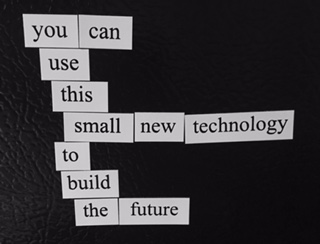
\includegraphics[width=90mm]{tree.jpg}
\caption{Rearranging these fridge magnets is equivalent to editing a TN document. The fridge magnet set that includes parenthesis is a poor seller.}
\end{figure}

\section{Conclusion}

TN is a useful base level notation for DSL's. TN supports clean multi-lingual composition, aligns well with version control paradigms, and has an unbreakable base grammar that allows for robust runtime editing.

With more tooling support and the discovery of more ETN's, TN will improve developer productivity and enable faster and easier creation and maintenance of software.

TTT also makes certain predictions about future discoveries, and provides a basis on which to make many more predictions.

\begin{thebibliography}{4}

\bibitem{Bray}
Bray, Tim, et al. "Extensible markup language (XML)." World Wide Web Consortium Recommendation REC-xml-19980210. http://www. w3. org/TR/1998/REC-xml-19980210 16 (1998): 16.

\bibitem{Crockford}
Crockford, Douglas. "The application/json media type for javascript object notation (json)." (2006).

\bibitem{JSON}
JSON.org. "Introducing JSON" (Accessed 3/2/2017). URL http://www.json.org/

\bibitem{Ooms}
Ooms, Jeroen. "The jsonlite package: A practical and consistent mapping between json data and r objects." arXiv preprint arXiv:1403.2805 (2014).

\end{thebibliography}

\ifCLASSOPTIONcaptionsoff
  \newpage
\fi

\end{document}
